\documentclass[varwidth=true, border=2pt]{standalone}

\usepackage{pgfplots}
\usepackage{tikz}
\usepackage{nicefrac}

\begin{document}
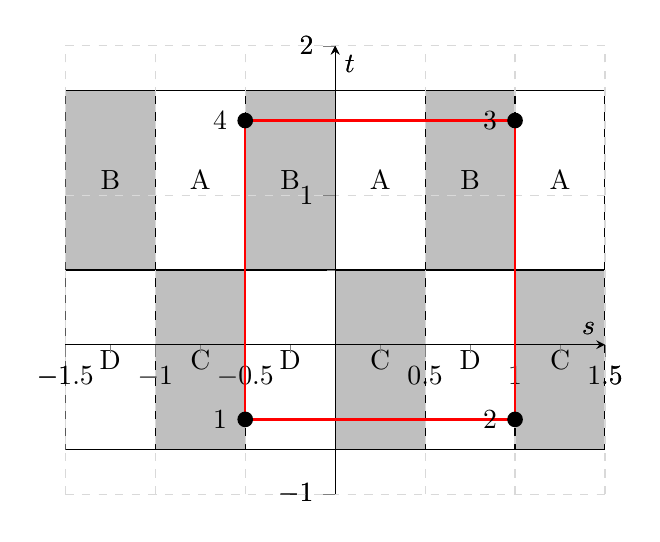
\begin{tikzpicture}
    \begin{axis}[
        legend pos=south west,
        axis x line=middle,
        axis y line=middle,
        grid = major,
        %width=9cm,
        %height=4.5cm,
        grid style={dashed, gray!30},
        xmin=-1.25,     % start the diagram at this x-coordinate
        xmax= 1.25,    % end   the diagram at this x-coordinate
        ymin=-0.75,     % start the diagram at this y-coordinate
        ymax= 1.75,   % end   the diagram at this y-coordinate
        axis background/.style={fill=white},
        xlabel=$s$,
        ylabel=$t$,
        %xticklabels={-2,-1.6,...,7},
        %yticklabels={-8,-7,...,8},
        tick align=outside,
        minor tick num=-3,
        enlargelimits=true,
        tension=0.08]

      \draw[fill=black!25] (axis cs:0.0,-.7) rectangle (axis cs:0.5,0.5) node[pos=.5] {C};
      \draw[fill=white]    (axis cs:0.5,-.7) rectangle (axis cs:1.0,0.5) node[pos=.5] {D};
      \draw[fill=white]    (axis cs:0.0,0.5) rectangle (axis cs:0.5,1.7) node[pos=.5] {A};
      \draw[fill=black!25] (axis cs:0.5,0.5) rectangle (axis cs:1.0,1.7) node[pos=.5] {B};
      \draw[fill=black!25] (axis cs:1.0,-.7) rectangle (axis cs:1.5,0.5) node[pos=.5] {C};
      \draw[fill=white]    (axis cs:1.0,0.5) rectangle (axis cs:1.5,1.7) node[pos=.5] {A};
      \draw[fill=black!25] (axis cs:-0.5,0.5) rectangle (axis cs:0.0,1.7) node[pos=.5] {B};
      \draw[fill=white]    (axis cs:-0.5,-.7) rectangle (axis cs:0.0,0.5) node[pos=.5] {D};
      \draw[fill=black!25] (axis cs:-0.5,-.7) rectangle (axis cs:-1.0,0.5) node[pos=.5] {C};
      \draw[fill=white]    (axis cs:-0.5,0.5) rectangle (axis cs:-1.0,1.7) node[pos=.5] {A};
      \draw[fill=black!25] (axis cs:-1.5,0.5) rectangle (axis cs:-1.0,1.7) node[pos=.5] {B};
      \draw[fill=white]    (axis cs:-1.5,-.7) rectangle (axis cs:-1.0,0.5) node[pos=.5] {D};

    \end{axis}
    \begin{axis}[
        axis x line=middle,
        axis y line=middle,
        grid = major,
        grid style={dashed, gray!30},
        xmin=-1.25,     % start the diagram at this x-coordinate
        xmax= 1.25,    % end   the diagram at this x-coordinate
        ymin=-0.75,     % start the diagram at this y-coordinate
        ymax= 1.75,   % end   the diagram at this y-coordinate
        xlabel=$s$,
        ylabel=$t$,
        %xticklabels={-2,-1.6,...,7},
        %yticklabels={-8,-7,...,8},
        tick align=outside,
        minor tick num=-3,
        enlargelimits=true,
        tension=0.08]
      \draw[red,thick] (axis cs:-0.5,-.5) rectangle (axis cs:1,1.5) node[pos=.5] {};

      \node[label={180:{1}},circle,fill,inner sep=2pt] at (axis cs:-0.5,-0.5) {};
      \node[label={180:{2}},circle,fill,inner sep=2pt] at (axis cs:1,-0.5) {};
      \node[label={180:{3}},circle,fill,inner sep=2pt] at (axis cs:1,1.5) {};
      \node[label={180:{4}},circle,fill,inner sep=2pt] at (axis cs:-0.5,1.5) {};
    \end{axis}
\end{tikzpicture}
\end{document}
